%%%%%%%%%%%%%%%%%%%%%%%%%%%%%%%%%%%%%%%%%
% Journal Article
% LaTeX Template
% Version 1.4 (15/5/16)
%
% This template has been downloaded from:
% http://www.LaTeXTemplates.com
%
% Original author:
% Frits Wenneker (http://www.howtotex.com) with extensive modifications by
% Vel (vel@LaTeXTemplates.com)
%
% License:
% CC BY-NC-SA 3.0 (http://creativecommons.org/licenses/by-nc-sa/3.0/)
%
%%%%%%%%%%%%%%%%%%%%%%%%%%%%%%%%%%%%%%%%%

%----------------------------------------------------------------------------------------
%	PACKAGES AND OTHER DOCUMENT CONFIGURATIONS
%----------------------------------------------------------------------------------------

\documentclass[twoside,twocolumn]{article}

\usepackage{blindtext} % Package to generate dummy text throughout this template 

\usepackage[sc]{mathpazo} % Use the Palatino font
\usepackage[T1]{fontenc} % Use 8-bit encoding that has 256 glyphs
\linespread{1.05} % Line spacing - Palatino needs more space between lines
\usepackage{microtype} % Slightly tweak font spacing for aesthetics

\usepackage[polish]{babel} % Language hyphenation and typographical rules

\usepackage[hmarginratio=1:1,top=32mm,columnsep=20pt]{geometry} % Document margins
\usepackage[hang, small,labelfont=bf,up,textfont=it,up]{caption} % Custom captions under/above floats in tables or figures
\usepackage{booktabs} % Horizontal rules in tables

\usepackage{lettrine} % The lettrine is the first enlarged letter at the beginning of the text

\usepackage{enumitem} % Customized lists
\setlist[itemize]{noitemsep} % Make itemize lists more compact

\usepackage{abstract} % Allows abstract customization
\renewcommand{\abstractnamefont}{\normalfont\bfseries} % Set the "Abstract" text to bold
\renewcommand{\abstracttextfont}{\normalfont\small\itshape} % Set the abstract itself to small italic text

\usepackage{titlesec} % Allows customization of titles
\renewcommand\thesection{\Roman{section}} % Roman numerals for the sections
\renewcommand\thesubsection{\roman{subsection}} % roman numerals for subsections
\titleformat{\section}[block]{\large\scshape\centering}{\thesection.}{1em}{} % Change the look of the section titles
\titleformat{\subsection}[block]{\large}{\thesubsection.}{1em}{} % Change the look of the section titles

\usepackage{fancyhdr} % Headers and footers
\pagestyle{fancy} % All pages have headers and footers
\fancyhead{} % Blank out the default header
\fancyfoot{} % Blank out the default footer
\fancyhead[C]{Algorytm Decyzyjny dla Rummikub $\bullet$ \today} % Custom header text
\fancyfoot[RO,LE]{\thepage} % Custom footer text

\usepackage{titling} % Customizing the title section

\usepackage{hyperref} % For hyperlinks in the PDF

%----------------------------------------------------------------------------------------
%	TITLE SECTION
%----------------------------------------------------------------------------------------

\setlength{\droptitle}{-4\baselineskip} % Move the title up

\pretitle{\begin{center}\Huge\bfseries} % Article title formatting
\posttitle{\end{center}} % Article title closing formatting
\title{Algorytm Decyzyjny dla Rummikub} % Article title
\author{%
\textsc{Aleksander Strzelecki}\\[1ex] % Your name
\normalsize Politechnika Gdańska \\ % Your institution
\normalsize \href{mailto:s179971@student.pg.edu.pl}{s179971@student.pg.edu.pl} % Your email address
}
\date{\today} % Leave empty to omit a date
\renewcommand{\maketitlehookd}{%
\begin{abstract}
\noindent
% Rummikub jest grą dla 2-4 osób. Gra składa się z 106 kości. Każda kość posiada numer od 1 do 13
% oraz jeden z kolorów(czarny, niebieski, pomarańczowy, czerwony). Każda kość występuje w dwóch egzemplarzach.
% Czyli mamy 13*4*2+2(jokery) = 106 kości. Joker może zastępować dowolną kość. Gracze zaczynają grę 
% z losowymi 14 koścmi. Reszta kości jest pulą, z której trzeba dobierać kości w przypadku braku ruchu przez 
% gracza. Celem gracza jest układanie kości na stole w serie (np. 1(czarny),2(czarny),3(czarny)) lub w grupy
% (1(czarny),1(czerwony),1(niebieski)). Seria lub grupa nie może liczyć mniej niż 3 kości. Gracz podczas ruchu może manipulować
% również aktualnymi seriami i grupami dostępnymi na stole. Gracz musi wykonać otwarcie (wyłożenie kości o sumie wartości 
% równej 30) w celu rozpoczęcia rozgrywki. Celem gry jest pozbycie się przez Gracza wszystkich swoich kości.
\end{abstract}
}

%----------------------------------------------------------------------------------------
% \usepackage{graphicx}
% \graphicspath{ {./resources/} }
\begin{document}

% Print the title
\maketitle

%----------------------------------------------------------------------------------------
%	ARTICLE CONTENTS
%----------------------------------------------------------------------------------------

\section{Wstęp}

% \lettrine[nindent=0em,lines=3]{L} orem ipsum dolor sit amet, consectetur adipiscing elit.


%------------------------------------------------

\section{Prace powiązane}

Rozwiązanie problemu Rummikuba zostało zaproponowane w \cite{Rijn:2016}. Algorytm wyliczał punktacje sumy ruchów, przy założeniu 
rozpoczęciu ruchu od konkretnej płytki. Polegało to na iteracji po wartościach rozpoczynających płytek od 1 do 13. W każdej iteracji układane były maksymalne 
ciągi przy wykorzystaniu płytek gracza o wartości z aktualnej iteracji. Z płytek o wartości z aktualnej iteracji, których nie można było już 
wykorzystać do rozbudowywania ciągów były wykorzystywane do rozbudowywania grup. Następnie wartości użytych płytek były sumowane i następowało 
rekurencyjne wywołanie próby rozbudowywania ciągów dla płytek o wartości z aktualnej iteracji + 1. Pojedyńcza iteracja kończyła się w momencie 
sprawdzenia możliwości rozbudowy ciągów z płytek o 
wartości = 13. Następnie cała procedura była wywoływana ponownie, ale dla wartości rozpoczynających płytek +1. W ten sposób uzyskiwaliśmy zestaw ruchów dający maksymalną punktację, jednak zakładając brak możliwośći manipulowania 
płytkami dostępnymi na stole.
% Algorytm decyzyjny przedstawiony w \cite{Rijn:2016} nie zakładał możliwości 
% manipulowania istniejącymi płytkami. Algorytm polegał na wyliczeniu punktacji ruchów w zależności od 
% płytki rozpoczynającej ruch. Następnie wybierany został zestaw ruchów o najlepszej punktacji.
%  Schemat szukania ruchów polegał na rozpoczęciu

Rummikub polega na wykonywaniu przekształceń na zbiorach liczbowych. Problem dobierania przekształceń został 
przedstawiony artykule \cite{Slagle:1963}, gdzie przekształcenia używane są do rozwiązywania całki symbolicznie.
Autor podzielił przekształcenia na korzystne i heurystyczne. Przekstałcenia korzystne wykonywane są pierwsze, a
heurystyczne w przypadku braku możliwości przekształcenia korzystnego. W miejscach, gdzie możliwe jest kilka 
przekształceń otrzymujemy rozgałęzienie. Następnie sprawdzana jest złożoność wyrażeń w otrzymanych gałęziach i 
do dalszego rozwiązywania wybierana jest zawsze gałąź z wyrażeniem o najmniejszej złożoności.

Podczas rozgrywki Rummikuba gracz znając aktualny stan planszy oraz dostępne płytki(stan gry) musi dobrać najlepsze 
przekształcenia(akcje). Po wykonaniu przekształceń gracz może oszacować wartość przekształceń sumując wartości pozbytych 
płytek(nagroda). Rozwiązanie tak zdefiniowanego problemu zostało przedstawione w \cite{Kaelbling:1996}. Agent(jednostka, której akcje dyktowane są przez algorytm) uczy się, które akcje są najlepsze 
w danym stanie gry, podczas rozgrywania kolejnych partii. W \cite{Kaelbling:1996} został również przedstawiony sposób na przechowywanie funkcji przejścia[Q(stan, akcja) -> nagroda] 
za pmocą sieci neuronowej. Połączenie sieci neuronowej z Q-learning tworzy algorytm Deep Q-learning.
% 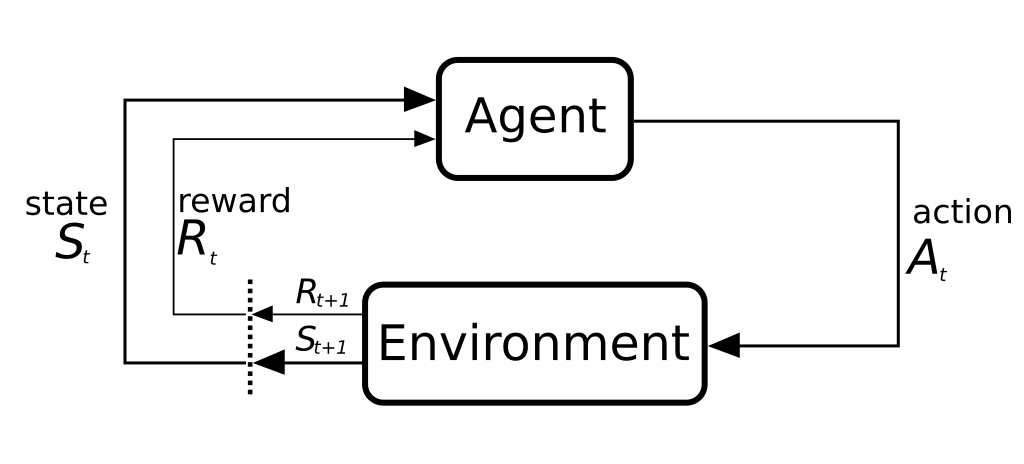
\includegraphics{Markov_diagram_v2.png}

Algorytm MinMax przedstawiony w \cite{Winston:1992} służył do dobierania ruchów gracza przy jednoczesnym uwzględnianiu możliwych ruchów przeciwnika. 
\cite{Winston:1992} przedstawia również zoptymalizowaną pod kątem prędkości działania wesję algorytmu MinMax - Alpha-Beta. Algorytm Alpha-Beta został użyty w maszynie  
Deep Blue\textsuperscript{\textregistered} \cite{Campbell:2002}, która w 1997 pokonała szachowego mistrza świata Garryego Kasparova. Dla przypadku, gdy w grze występuje 
element losowy(np. rzut kością, wylosowanie płytek w Rummikubie) został opracowany algorytm Expectiminimax \cite{Stuart:2009}. Algorytm sumuje wartości ruchów pomnożone 
przez prawdopodobieństwa ich wystąpień.

%------------------------------------------------
\section{Proponowane rozwiązanie}
%------------------------------------------------
\section{Wyniki}
%------------------------------------------------

\section{Podsumowanie}

%----------------------------------------------------------------------------------------
%	REFERENCE LIST
%----------------------------------------------------------------------------------------

\bibliographystyle{plain}
\bibliography{refs}

%----------------------------------------------------------------------------------------

\end{document}
